% This must be in the first 5 lines to tell arXiv to use pdfLaTeX, which is strongly recommended.
\pdfoutput=1
% In particular, the hyperref package requires pdfLaTeX in order to break URLs across lines.

\documentclass[11pt]{article}

% Remove the "review" option to generate the final version.
% \usepackage[review]{ACL2023}
\usepackage{ACL2023}

% Standard package includes
\usepackage{times}
\usepackage{latexsym}

% For proper rendering and hyphenation of words containing Latin characters (including in bib files)
\usepackage[T1]{fontenc}
% For Vietnamese characters
% \usepackage[T5]{fontenc}
% See https://www.latex-project.org/help/documentation/encguide.pdf for other character sets

% This assumes your files are encoded as UTF8
\usepackage[utf8]{inputenc}
\usepackage{tcolorbox}
\tcbuselibrary{breakable}

% This is not strictly necessary, and may be commented out.
% However, it will improve the layout of the manuscript,
% and will typically save some space.
\usepackage{microtype}

% This is also not strictly necessary, and may be commented out.
% However, it will improve the aesthetics of text in
% the typewriter font.
\usepackage{inconsolata}
\usepackage{mymathdef}

\newcommand{\FT}[0]{\includegraphics[width=.018\textwidth]{res/fire_emoji_apple.png}}
\newcommand{\FE}[0]{\includegraphics[width=.018\textwidth]{res/snowflake_emoji_apple.png}}



% If the title and author information does not fit in the area allocated, uncomment the following
%
%\setlength\titlebox{<dim>}
%
% and set <dim> to something 5cm or larger.

\title{SoftCoT: Soft Chain-of-Thought for Efficient Reasoning with LLMs}

% Author information can be set in various styles:
% For several authors from the same institution:
% \author{Author 1 \and ... \and Author n \\
%         Address line \\ ... \\ Address line}
% if the names do not fit well on one line use
%         Author 1 \\ {\bf Author 2} \\ ... \\ {\bf Author n} \\
% For authors from different institutions:
% \author{Author 1 \\ Address line \\  ... \\ Address line
%         \And  ... \And
%         Author n \\ Address line \\ ... \\ Address line}
% To start a seperate ``row'' of authors use \AND, as in
% \author{Author 1 \\ Address line \\  ... \\ Address line
%         \AND
%         Author 2 \\ Address line \\ ... \\ Address line \And
%         Author 3 \\ Address line \\ ... \\ Address line}

% \author{First Author \\
%   Affiliation / Address line 1 \\
%   Affiliation / Address line 2 \\
%   Affiliation / Address line 3 \\
%   \texttt{email@domain} \\\And
%   Second Author \\
%   Affiliation / Address line 1 \\
%   Affiliation / Address line 2 \\
%   Affiliation / Address line 3 \\
%   \texttt{email@domain} \\}
\author{
Yige Xu${^{1,2}}$\thanks{\ \  The first two authors contributed equally.}, Xu Guo$^{1,*}$\footnotemark[2], Zhiwei Zeng$^1$\thanks{\ \  Corresponding authors.}, Chunyan Miao$^{1,2}$ \\
$^1$Joint NTU-UBC Research Centre of Excellence in Active Living for the Elderly \\
$^2$College of Computing and Data Science \\
Nanyang Technological University, Singapore \\
\texttt{\{yige002,xu008\}@e.ntu.edu.sg}, \texttt{\{zhiwei.zeng,ascymiao\}@ntu.edu.sg}
%corresponding
}

\begin{document}
\maketitle
\begin{abstract}
Chain-of-Thought (CoT) reasoning enables Large Language Models (LLMs) to solve complex reasoning tasks by generating intermediate reasoning steps. However, most existing approaches focus on hard token decoding, which constrains reasoning within the discrete vocabulary space and may not always be optimal. While recent efforts explore continuous-space reasoning, they often require full-model fine-tuning and suffer from catastrophic forgetting, limiting their applicability to state-of-the-art LLMs that already perform well in zero-shot settings with a proper instruction. To address this challenge, we propose a novel approach for continuous-space reasoning that does not require modifying the LLM. Specifically, we employ a lightweight fixed assistant model to generate instance-specific soft thought tokens speculatively as the initial chain of thoughts, which are then mapped into the LLM’s representation space via a trainable projection module. Experimental results on five reasoning benchmarks demonstrate that our method enhances LLM reasoning performance through supervised, parameter-efficient fine-tuning.
\end{abstract}

\section{Introduction}


In recent years, Large Language Models (LLMs) have become a cornerstone in Natural Language Processing (NLP), exhibiting advanced natural language understanding and generation~\cite{DBLP:conf/nips/BrownMRSKDNSSAA20,chowdhery2023palm,openai2023gpt4,dubey2024llama,DBLP:journals/corr/abs-2412-15115}.
Scaling model sizes has not only improved instruction-following~\cite{DBLP:conf/nips/KojimaGRMI22} but also triggered emergent reasoning abilities, as first evidenced by chain-of-thought (CoT) prompting~\cite{DBLP:conf/nips/Wei0SBIXCLZ22}.
CoT prompts LLMs to generate intermediate reasoning steps before providing the final answer, which not only enhances interpretability but also improves a range of reasoning-intensive tasks~\cite{DBLP:conf/iclr/0001Z0S23,DBLP:journals/corr/abs-2409-12183}. It has inspired many advanced prompting frameworks, marking a paradigm shift from scaling training-time compute~\cite{DBLP:conf/nips/KojimaGRMI22} to scaling inference-time compute~\cite{DBLP:conf/iclr/0002WSLCNCZ23,DBLP:conf/nips/YaoYZS00N23} to further boost LLM performance.

Nevertheless, CoT's effectiveness depends on the quality of intermediate thoughts, as the auto-regressive generation process can propagate errors. To mitigate this challenge, methods like self-consistency~\cite{DBLP:conf/iclr/0002WSLCNCZ23} generate multiple reasoning paths, while Tree-of-Thought~\cite{DBLP:conf/nips/YaoYZS00N23} and Graph-of-Thought~\cite{DBLP:conf/aaai/BestaBKGPGGLNNH24} frameworks organize these paths to select higher-quality steps. Despite these improvements, such methods are computationally inefficient due to the need for extensive thought sampling.

To enhance CoT efficiency, recent research explores skipping the decoding of hard tokens at intermediate steps. Methods like Continuous CoT \citep{DBLP:journals/corr/abs-2412-13171} and Coconut \citep{DBLP:journals/corr/abs-2412-06769} conduct reasoning in a continuous space by using latent representations instead of discrete token sequences.
Their results have shown to be superior to long-sequence discrete reasoning chains using only a short length of continuous representation. Yet, these methods require full-model fine-tuning, which incurs substantial computational costs, risks catastrophic forgetting, and limits their transferability across tasks.

We empirically observe that supervised fine-tuning of the LLaMA3.1-8B~\cite{dubey2024llama} model with a language modeling objective on reasoning tasks (which is employed by both Coconut and CCoT) can lead to performance degradation compared with the zero-shot settings. We conjecture that this is due to catastrophic forgetting, a phenomenon also observed by \citet{DBLP:journals/corr/abs-2401-05605} and \citet{DBLP:journals/corr/abs-2411-15382}. Thus, the methodologies of Coconut, which is based on GPT-2~\cite{radford2019language}, and CCoT, which is built upon LLaMA2-7B~\cite{touvron2023llama2}, may not be directly applicable to more recent models such as LLaMA3.1-8B. Therefore, it is crucial to explore alternative methodologies that mitigate catastrophic forgetting while effectively leveraging continuous reasoning techniques in large-scale, instruction-tuned models, which is the main research question of this work.

To mitigate catastrophic forgetting, a straightforward approach is to freeze the backbone LLM and instead optimize an external model for reasoning. Inspired by prompt tuning~\cite{DBLP:conf/emnlp/LesterAC21} and speculative decoding \citep{DBLP:conf/icml/LeviathanKM23}, we propose an approach that utilizes an auxiliary small assistant model to generate a sequence of ``thought'' tokens conditioned on a task instruction followed by a specific instance~\cite{DBLP:conf/nips/LiPHGGY23,DBLP:conf/icml/ShaoGSHDC23}. These tokens serve as instance-specific prompts to boost LLM's inference. Such an auxiliary prompting mechanism dynamically adapts to different reasoning tasks, thereby improving generalization while preserving the pre-trained knowledge of the LLM.

To facilitate reasoning in a continuous space, we use soft thought tokens (i.e., the last-layer hidden states from the small assistant model before mapping to the vocabulary space) instead of discrete tokens. This ensures reasoning remains within the continuous latent space. However, a representational gap between the assistant model and the LLM may hinder effective knowledge transfer. To bridge this gap, we train a projection module to map the soft thought tokens generated by the assistant model to the LLM's representation space. Training the projection module for each task can be seen as \textit{soft prompt tuning} for the LLM. The overall \underline{\bf Soft} thoughts for \underline{\bf CoT} (SoftCoT) reasoning framework is illustrated in Figure~\ref{fig:softcot-methodology-overview}.

To evaluate our proposed SoftCoT, we conduct experiments on five reasoning benchmarks and two state-of-the-art LLM architectures. The five benchmarks we choose include mathematical reasoning, commonsense reasoning, and symbolic reasoning. For further exploration, we create a hard version of the ASDiv dataset~\cite{DBLP:conf/acl/MiaoLS20}, which requires stronger mathematical reasoning ability. The new dataset is named ``ASDiv-Aug'' in this paper. Experimental results show that SoftCoT consistently improves accuracy on both public datasets and our augmented ASDiv-Aug dataset, demonstrating the effectiveness of SoftCoT in enhancing LLM's reasoning performance. Moreover, SoftCoT employs parameter-efficient fine-tuning, effectively mitigating catastrophic forgetting seen in full-model fine-tuning. Our results highlight the effectiveness of using an assistant model to generate soft thoughts for enhancing LLMs' reasoning capabilities while preserving their pre-trained knowlegde.



\begin{figure*}[!thp]
  \centering
  \includegraphics[width=0.97\textwidth]{main-figure.pdf}
\caption{A comparison of SoftCoT, vanilla Chain-of-Thought, and Coconut.}\label{fig:softcot-methodology-overview}
\end{figure*}


\section{Related Works}

Early research on chain-of-thought (CoT) reasoning can be traced back to \citet{DBLP:conf/nips/Wei0SBIXCLZ22}, who first introduced a prompting strategy that guides LLMs through decomposed intermediate reasoning steps using few-shot exemplars. Concurrently, \citet{DBLP:conf/nips/KojimaGRMI22} demonstrated that LLMs are capable of zero-shot CoT reasoning by simply appending the phrase ``Let's think step by step'' to the prompt template. This discovery underscored the latent reasoning abilities of LLMs, even in the absence of explicit demonstrations.

Building upon these foundational works, the NLP community has extensively explored the potential of CoT reasoning. As summarized by \citet{DBLP:conf/acl/ChuCCYH0P00L24}, recent advancements in CoT methods can be broadly categorized into three areas: (1) {\it Prompt Construction}, which aims to optimize prompts for improved CoT reasoning \cite{DBLP:conf/nips/Wei0SBIXCLZ22,DBLP:conf/nips/KojimaGRMI22,DBLP:conf/iclr/0001Z0S23}; (2) {\it Topological Variants}, which leverage structured representations such as trees and graphs to enhance CoT reasoning~\cite{DBLP:conf/nips/YaoYZS00N23,DBLP:conf/aaai/BestaBKGPGGLNNH24}; and (3) {\it Enhancement Methods}, which introduce external strategies to further improve CoT reasoning, such as question decomposition~\cite{DBLP:conf/iclr/ZhouSHWS0SCBLC23} and self-consistency decoding \cite{DBLP:conf/iclr/0002WSLCNCZ23}. Despite the effectiveness of these approaches, the majority of existing CoT methods rely on discrete token-by-token generation, which imposes inherent constraints and limits their expressiveness.

To address the limitations of discrete language space, an effective approach is to leverage continuous representation space for reasoning. Coconut~\cite{DBLP:journals/corr/abs-2412-06769} introduces a Chain-of-Continuous-Thought, while CCoT~\cite{DBLP:journals/corr/abs-2412-13171} employs Compressed Chain-of-Thought, generating content-rich and continuous contemplation tokens. Heima~\cite{DBLP:journals/corr/abs-2501-19201} further advances this idea by utilizing a single continuous vector to represent compressed reasoning tokens in multi-modal tasks. However, both Coconut and CCoT rely on a language modeling objective for supervised fine-tuning, which is infeasible for state-of-the-art LLMs due to the catastrophic forgetting problem. Moreover, Heima underperforms compared to its backbone model, LLaVA-CoT~\cite{DBLP:journals/corr/abs-2411-10440}. These challenges underscore the need to develop methodologies that mitigate catastrophic forgetting in the application of continuous-space CoT reasoning.


\section{Methodology}

\subsection{Problem Definition and Notations}
\label{sec:softcot-methodology-problem-def}

Given a question $\cQ=[q_1,q_2,\cdots,q_{|\cQ|}]$, the CoT reasoning will solve the problem on the following two steps: (1) Auto-regressively generate a list of rationale steps $\cR=[r_1,r_2,\cdots,r_{|\cR|}]$ according to the question; (2) Auto-regressively generate the answer $\cA=[a_1,a_2,\cdots,a_{|\cA|}]$ according to the question as well as the rationale steps. The generation process can be described as:
\begin{align}
  r_{i+1}&=\mathrm{LLM}(\cQ;\cR_{\le i}),\\\nonumber
  a_{j+1}&=\mathrm{LLM}(\cQ;\cR;\cA_{\le j}),
\end{align}
where $\mathrm{LLM}(\cdot)$ indicates a large language model, $\cR_{\le i}=[r_1,\cdots,r_i]$ indicates the previous generated $i$ reasoning tokens, and $\cA_{\le j}=[a_1,\cdots,a_j]$ indicates the previous generated $j$ answer tokens.

The majority of recent works~\cite{DBLP:conf/iclr/0001Z0S23,DBLP:conf/iclr/ZhouSHWS0SCBLC23,DBLP:conf/nips/YaoYZS00N23} focus on generating discrete hard tokens in $\cR$, which is named as ``{\bf Hard-CoT}'' in this paper. On contrast, some recent works~\cite{DBLP:journals/corr/abs-2412-06769,DBLP:journals/corr/abs-2412-13171} focus on the continuous representations ({\it a.k.a} latent space) of $\cR$, which is named as ``{\bf Soft-CoT}'' in this paper.

In this paper, we mannually define some rules (e.g., regular expression matching) to extract the framework answer $\hat{\cA}$ from the answer $\bar{\cA}$ generated by the LLM. Then we compute the accuracy of $\hat{\cA}$ comparing with the ground-truth answer $\cA$.


\subsection{Overview of the SoftCoT Framework}

SoftCoT is a novel framework designed to enhance reasoning capabilities in large language models (LLMs). Given an input question $\cQ$, the framework produces both a sequence of reasoning steps $\cR$ and the final answer $\cA$. SoftCoT consists of three key components: the soft thought token generation module, the projection module, and the CoT reasoning module. The overall architecture is illustrated in Figure~\ref{fig:softcot-methodology-overview}(a).

The soft thought token generation module is inspired by prompt tuning techniques~\cite{DBLP:conf/emnlp/LesterAC21}. In conventional prompt tuning, learnable prompts facilitate the retrieval of knowledge stored within the LLM~\cite{xu-etal-2023-efficient}. In SoftCoT, soft thought tokens are generated by an assistant language model, which is typically smaller than the backbone LLM (e.g., LLaMA-3.2-1B-Instruct as the assistant model and LLaMA-3.1-8B-Instruct as the backbone model).

A key challenge in this setup is that the assistant model can only generate discrete token sequences as input to the backbone LLM, which imposes constraints and may not always yield optimal prompts. To address this limitation, we introduce continuous soft thought tokens that enable more expressive and flexible prompting. However, a representation gap exists between the assistant model and the backbone LLM, necessitating an intermediate transformation.

To bridge this gap, the projection module maps the soft thought tokens' representations into a space more compatible with the backbone LLM. This ensures that the soft thought tokens effectively guide the reasoning process.

Finally, the CoT reasoning module leverages both the learned soft thought tokens and word embeddings to generate intermediate reasoning steps $\bar{\cR}$ and the final answer $\bar{\cA}$. The model is trained using a language modeling objective, optimizing the learnable parameters across the rationale steps and the answer spans.


\subsection{Prompt Tuning for CoT Reasoning}

Prompt tuning for CoT reasoning aims to optimize the structure and content of the prompt template to enhance the reasoning capabilities of a large language model (LLM). This process can be mathematically formulated as follows:
\begin{align}
  \hat{y}&=\mathrm{LLM}\big(P_{\bp}(x)\big),\\\nonumber
  \bp^*&=\arg \min_{\bp} \cL(\hat{y},y),
\end{align}
where $\hat{y}$ represents the predicted output, $x$ denotes the input sequence, and $P_{\bp}(x)$ is the input augmented with a prompt $\bp$. The objective function $\cL(\cdot)$ measures the discrepancy between the model's prediction $\hat{y}$ and the ground-truth label $y$. The primary goal of prompt tuning is to determine an optimal prompt configuration that effectively guides the LLM to perform CoT reasoning with improved accuracy and interpretability.

A straightforward yet effective approach to optimizing prompts involves leveraging an auxiliary assistant model to generate instance-specific prompts, which provide contextual hints or question summaries to facilitate reasoning~\cite{DBLP:conf/nips/LiPHGGY23,DBLP:conf/icml/ShaoGSHDC23}. In this framework, the prompt $\bp$ can be decomposed into two components: (1) a fixed, task-specific prompt $\bp_{\FE}$,  which remains constant across all instances and encodes general problem-solving heuristics, and (2) a learnable, instance-specific prompt $\bp_{\FT}$, which dynamically adapts to each input instance to provide tailored guidance.

Given the rapid advancements in LLMs, many LLMs are capable of solving complex reasoning tasks under zero-shot settings. Instead of fine-tuning the assistant model for each task, we adopt a more efficient strategy by employing a relatively small, frozen language model to generate $\bp_{\FT}$. This approach not only reduces computational costs but also ensures stability and generalization across different problem domains. By systematically integrating instance-specific prompting with fixed task-specific instructions, this method enhances the LLM's reasoning process while maintaining adaptability to various contexts.


\subsection{Soft Thought Tokens for CoT Reasoning}

One of the advantages of Hard-CoT is that the generated discrete tokens can be tokenized by the LLMs, which does not require a external mapping module. However, there are two main limitations of Hard-CoT: (1) The decoded token space is discrete, which is constrained and sometimes not optimal; (2) The gradient cannot backpropagate to the assistant model since the decoding process cut off the gradient information. A convincing solution is replace the hard tokens to soft thought tokens.

\paragraph{Generating Soft Thought Tokens with an Assistant Model}

To generate instance-specific soft thoughts, we utilize an auxiliary assistant model that produces soft thoughts based on the given reasoning task. The input to the assistant model, denoted as $\bx_{\mathrm{assist}}$, consists of three main components:
\begin{align}
  \bx_{\mathrm{assist}}=\big[\cI,\cQ,\texttt{[UNK]}_{1:N}\big],\\\nonumber
\end{align}
where
\begin{itemize}
  \item $\cI$ represents the instructional context provided to the assistant model, guiding it on how to generate relevant thoughts.
  \item $\cQ$ denotes the reasoning question that the primary LLM will solve, which has been defined in Section~\ref{sec:softcot-methodology-problem-def}.
  \item $N$ \texttt{[UNK]} tokens serve as placeholders for the soft thoughts.
\end{itemize}

Once the input sequence is constructed, the assistant model processes it, and the soft thought tokens are obtained as follows:
\begin{align}
  \bh^{\mathrm{assist}}&=\mathrm{Assistant}(\bx_{\mathrm{assist}}),\\\nonumber
  \bt_{\mathrm{assist}}&=\bh^{\mathrm{assist}}_{|\cI|+|\cQ|+1:|\cI|+|\cQ|+N}.
\end{align}
Here $\bh^{\mathrm{assist}}$ denotes the final-layer hidden states of the assistant model, and $\bt_{\mathrm{assist}}$ corresponds to the segment of $\bh^{\mathrm{assist}}$ associated with the $N$ \texttt{[UNK]} tokens. This extracted representation serves as the instance-specific soft thoughts, dynamically adapting to the input reasoning question.

\paragraph{Projection Module}

Since there exist both a representation gap and a dimensional gap between the assistant language model and the primary LLM, a direct utilization of $\bt_{\mathrm{assist}}$ may lead to suboptimal performance. The assistant model and the LLM often operate in different embedding spaces, with distinct hidden state distributions and dimensionalities. To bridge this gap, we introduce a projection module that maps the assistant-generated soft thoughts $\bt_{\mathrm{assist}}$ from the assistant model's embedding space to the LLM's embedding space:
\begin{align}
  \bt_{\FT}=\mathrm{Linear}_{\theta}(\bt_{\mathrm{assist}}),\label{eq:softcot-projection}
\end{align}
where $\mathrm{Linear}_{\theta}:\mathbb{R}^{d_\mathrm{assist}}\to \mathbb{R}^{d_\mathrm{LLM}}$ is a trainable projection layer parameterized by $\theta$. This layer ensures that the assistant-generated soft thoughts are transformed into a suitable format for the LLM, preserving relevant semantic information while adapting to the LLM’s feature space.

By incorporating this projection module, we effectively mitigate discrepancies between the assistant model and the LLM, enabling smooth integration of instance-specific thoughts into the CoT reasoning process. This design ensures that the learned thought tokens are both informative and compatible, thereby enhancing the overall reasoning performance of the LLM.

\paragraph{LLM Reasoning with Soft CoT}
With instance-specific soft thought tokens generated by the assistant model and mapped to the LLM's embedding space, we proceed to the final step: applying these soft thoughts to aid LLMs in CoT reasoning.

The input to the LLM, denoted as $\bx_{\mathrm{LLM}}$, follows a structure similar to that of  $\bx_{\mathrm{assist}}$:
\begin{align}
   \bx_{\mathrm{LLM}}=\big[\bp_{\FE},\cQ,\bt_{\FT}\big],\label{eq:softcot-llm-iput-def}
\end{align}
where
\begin{itemize}
  \item $\bp_{\FE}$ is the task-specific instruction, which is a fixed prompt shared across all instances of the same task. It provides general problem-solving heuristics and instructions relevant to the reasoning task.
  \item $\bt_{\FT}$ is the instance-specific soft thoughts computed by Eq~\eqref{eq:softcot-projection}. This component dynamically adapts soft thought tokens to each input question, enhancing contextual understanding.
\end{itemize}

With this structured input, the LLM generates step-by-step reasoning chains, following the principles of CoT reasoning. The reasoning process unfolds by systematically applying logical deductions or problem-solving heuristics, ultimately leading to the generation of the final answer:
\begin{align}
  \bar{\cR}&=\mathrm{LLM}(\bx_{\mathrm{LLM}}),\\\nonumber
  \bar{\cA}&=\mathrm{LLM}(\bx_{\mathrm{LLM}},\bar{\cR}),\\\nonumber
  \hat{\cA}&=\cE(\bar{\cA}),
\end{align}
where $\cE(\cdot)$ is mannual rules for answer extraction.

By integrating both fixed task-specific instructions and instance-specific soft thought tokens, our approach enables the LLM to systematically decompose complex reasoning tasks while leveraging auxiliary knowledge provided by the assistant model. The structured input ensures that the LLM benefits from both general domain knowledge and tailored instance-level guidance, ultimately improving its reasoning effectiveness.

\paragraph{Parameter-Efficient Training}

In this work, we focus on reasoning tasks that include annotated reasoning steps, which provide explicit intermediate reasoning trajectories leading to the final answer. To effectively train the model, we employ the standard language modeling objective (also known as next-token prediction) to supervise the generation of soft thoughts. During the training stage, the input sequence is structured as follows:
\begin{align}
   \bx_{\mathrm{train}}=\big[\bp_{\FE},\cQ,\bt_{\FT},\cR,\cA\big].
\end{align}

To effectively learn the soft thoughts, we apply the negative log-likelihood (NLL) loss over the reasoning steps and the answer span. Specifically, we mask the tokens before the intermediate reasoning steps to prevent the model from directly relying on them during loss computation. Instead, the model is trained to generate the reasoning steps $\cR$ and final answer $\cA$ in an autoregressive manner.



\section{Experiments}

\subsection{Datasets}

We conduct experiments on five reasoning datasets spanning three categories of reasoning: mathematical reasoning, commonsense reasoning, and symbolic reasoning. For mathematical reasoning, we utilize {\bf GSM8K}~\cite{cobbe2021gsm8k}, {\bf ASDiv}~\cite{DBLP:conf/acl/MiaoLS20}, and {\bf AQuA}~\cite{DBLP:conf/acl/LingYDB17}. For commonsense reasoning, we employ {\bf StrategyQA}~\cite{DBLP:journals/tacl/GevaKSKRB21}. For symbolic reasoning, we use {\bf Date Understanding}~\cite{DBLP:journals/tmlr/SrivastavaRRSAF23} from the BIG-benchmark.

Given that LLaMA-3.1-8B-Instruct is a well-trained LLM, we augment the ASDiv dataset to ensure that the model encounters novel instances. Specifically, we replicate each instance five times and systematically extract and replace numerical values in the questions with randomly selected alternatives. This augmentation is designed to evaluate the model's reasoning capability rather than its ability to recognize patterns from memorized data. The augmented dataset is named as ``{\bf ASDiv-Aug}'' in the following part of this paper. All detail statistics of the datasets is shown in Table~\ref{table:softcot-experiment-dataset}.

\begin{table*}[t!]
    \centering
    \tabcolsep 6.0pt
    \begin{tabular}{l|c c c c }
    \toprule
    Dataset & Task Type & Answer Type & \# Train samples & \# Evaluation samples \\
    \midrule
    GSM8K & \multirow{3}{*}{Mathematical} & Number & 7,473 & 1,319\\
    ASDiv-Aug & ~ & Number & 4,183 & 1,038 \\
    AQuA & ~ & Option & 97,467 & 254 \\
    \midrule
    StrategyQA & Commonsense & Yes/No & 1,832 & 458 \\
    \midrule
    DU & Symbolic & Option & - & 250 \\
    \bottomrule
\end{tabular}
    \caption{Summary statistics of fiva datasets we used. ``-'' indicates that there is no training samples available.}\label{table:softcot-experiment-dataset}
\end{table*}


\subsection{Baselines}
\label{sec:softcot-exp-baselines}
We consider the following baselines:

\paragraph{Coconut}~\cite{DBLP:journals/corr/abs-2412-06769}. It enables LLMs to reason in a continuous latent space by iteratively feeding hidden states as input embeddings, allowing for more efficient and flexible multi-path reasoning compared to traditional language-based chain-of-thought methods.

\paragraph{Zero-Shot CoT} To evaluate whether our trained model has performance degration after supervised fine-tuning, we apply zero-shot CoT based on the prompt templates from \citet{DBLP:journals/corr/abs-2409-12183}.


\paragraph{Zero-Shot CoT-Unk} We directly add some \texttt{[UNK]} tokens to represent the un-tuned prompts for CoT reasoning. This baseline exams the effectiveness of the tuned prompts.

\paragraph{Zero-Shot Assist-CoT} We directly require the assistant model generates some hard prompt tokens for CoT reasoning. This baseline exams the effectiveness of the tuned soft prompts.



\begin{table*}[t!]
\setlength{\tabcolsep}{4pt}
    \centering
    \begin{tabular}{l| c c c | c | c | c c c c c}
    \toprule
    \multirow{2}{*}{Model} & GSM8K & ASDiv-Aug & AQuA & StrategyQA & DU & Avg. \\
    \cline{2-7}
    ~ & \multicolumn{3}{c|}{Mathematical} & Commonsense & Symbolic \\
    \midrule
    {\it GPT-2} & \\
    Coconut~\cite{DBLP:journals/corr/abs-2412-06769}
    & 34.10$^{*}_{\pm \text{1.50}}$ & 38.92$^{\dagger}_{\pm \text{0.00}}$ & 22.83$^{\dagger}_{\pm \text{0.00}}$ & - & - & - \\
    \midrule
    \midrule
    {\it LLaMA-3.1-8B-Instruct}\\
    Zero-Shot CoT
    & 79.61$_{\pm \text{0.81}}$ & 86.78$_{\pm \text{0.63}}$ & 54.65$_{\pm \text{2.43}}$ & 65.63$_{\pm \text{3.31}}$ & 54.40$_{\pm \text{2.40}}$ & 68.21 \\
    Zero-Shot CoT-Unk
    & 79.95$_{\pm \text{0.59}}$ & 86.90$_{\pm \text{0.41}}$ & 55.28$_{\pm \text{1.88}}$ & 66.16$_{\pm \text{2.70}}$ & 54.16$_{\pm \text{1.46}}$ & 68.49 \\
    Zero-Shot Assist-CoT
    & 80.76$_{\pm \text{1.53}}$ & 86.96$_{\pm \text{0.46}}$ & 55.83$_{\pm \text{2.98}}$ & 66.55$_{\pm \text{3.99}}$ & 58.24$_{\pm \text{3.56}}$ & 69.67 \\
    \midrule
    Coconut~\cite{DBLP:journals/corr/abs-2412-06769}$^{\dagger}$
    & 76.12$_{\pm \text{0.00}}$ & 86.80$_{\pm \text{0.00}}$ & 53.15$_{\pm \text{0.00}}$ & - & - & - \\
    {\bf SoftCoT (Ours)}
    & {\bf 81.03$_{\pm \text{0.42}}$} & {\bf 87.19$_{\pm \text{0.40}}$} & {\bf 56.30$_{\pm \text{1.67}}$} & {\bf 69.04$_{\pm \text{1.23}}$} & {\bf 59.04$_{\pm \text{1.93}}$} & {\bf 70.52} \\
    \bottomrule
\end{tabular}
\caption{Model comparison with baselines. ``DU'' indicates the Date Understanding~\cite{DBLP:journals/tmlr/SrivastavaRRSAF23} dataset. The first row is under the backbone of GPT-2~\cite{radford2019language} as backbone. The following rows are under the backbone of LLaMA-3.1-8B-Instruct~\cite{dubey2024llama}. The last two rows are models trained via the language modeling objective. We run for 5 random seeds and report the average accuracy as well as the standard variance. ``*'' indicates that the accuracy is reported by \citet{DBLP:journals/corr/abs-2412-06769}. ``$^{\dagger}$'' indicates the results that we modify and run the official code of Coconut. ${\pm \text{0.00}}$ indicates that we only run once for baseline results.
\label{table:softcot-result-comparison}}
\end{table*}


\begin{table*}[t!]
\setlength{\tabcolsep}{4pt}
    \centering
    \begin{tabular}{l| c c c | c | c | c c c c c}
    \toprule
    \multirow{2}{*}{Model} & GSM8K & ASDiv-Aug & AQuA & StrategyQA & DU & Avg. \\
    \cline{2-7}
    ~ & \multicolumn{3}{c|}{Mathematical} & Commonsense & Symbolic \\
    \midrule
    Zero-Shot CoT
    & 83.70$_{\pm \text{0.78}}$ & 87.19$_{\pm \text{0.28}}$ & 64.53$_{\pm \text{3.27}}$ & 49.65$_{\pm \text{3.18}}$ & 66.40$_{\pm \text{2.26}}$ & 70.29 \\
    Zero-Shot CoT-Unk
    & 84.12$_{\pm \text{0.71}}$ & 86.94$_{\pm \text{0.89}}$ & 64.72$_{\pm \text{2.06}}$ & 50.74$_{\pm \text{1.90}}$ & 66.48$_{\pm \text{1.43}}$ & 70.60 \\
    Zero-Shot Assist-CoT
    & 84.85$_{\pm \text{0.35}}$ & 88.63$_{\pm \text{1.05}}$ & 64.96$_{\pm \text{2.83}}$ & 52.71$_{\pm \text{2.65}}$ & 67.04$_{\pm \text{2.84}}$ & 71.64 \\
    \midrule
    {\bf SoftCoT (Ours)}
    & {\bf 85.81$_{\pm \text{1.82}}$} & {\bf 88.90$_{\pm \text{1.01}}$} & {\bf 72.44$_{\pm \text{2.19}}$} & {\bf 60.61$_{\pm \text{1.55}}$} & {\bf 67.52$_{\pm \text{2.92}}$} & {\bf 75.06} \\
    \bottomrule
\end{tabular}
\caption{Model performance using Qwen2.5-7B-Instruct.
\label{table:softcot-generation-to-qwen2.5}}
\end{table*}

\section{Results and Discussions}

\subsection{Comparison with Baselines}

To evaluate SoftCoT, we compare its performance against the baselines introduced in Section~\ref{sec:softcot-exp-baselines}. The results are summarized in Table~\ref{table:softcot-result-comparison}:

\noindent (1) {\bf Coconut is not applicable to larger language models}: We modify and run the official implementation of Coconut, adapting it to LLaMA-3.1-8B-Instruct. Our findings indicate that Coconut exhibits performance degradation following supervised fine-tuning with the language modeling objective, which can be attributed to the catastrophic forgetting phenomenon. This observation aligns with findings from prior studies, including \citet{DBLP:journals/corr/abs-2401-05605} and \citet{DBLP:journals/corr/abs-2411-15382}, which have reported similar issues.

\noindent (2) {\bf Incorporating \texttt{[UNK]} tokens mitigates performance variance}: We examined the effect of directly adding \texttt{[UNK]} tokens as thoughts $\bt_{\FT}$ in Eq.~\eqref{eq:softcot-llm-iput-def}. The results demonstrate a slight improvement in overall performance and a reduction in variance. The \texttt{[UNK]} token, also known as the ``pause token''~\cite{DBLP:conf/iclr/GoyalJRMKN24}, appears to expand the model's computational capacity, leading to more stable and consistent outputs.

\noindent (3) {\bf Assistant model is effective to facilitate CoT reasoning}: We utilize instruction to require the assistant model generate some hard prompts, which can be regarded as the initial thoughts for CoT reasoning. Experiment results show that although it has a larger variance than CoT-Unk, it facilitates the LLM for more diverse CoT generation, which leads to the performance improvement from 68.49 to 69.67 in average.

\noindent (4) {\bf SoftCoT consistently benefits from the supervised fine-tuning}: Overall, our proposed SoftCoT consistently outperforms baselines across all five reasoning datasets, involving the mathematical reasoning, the commonsense reasoning, and the symbolic reasoning. The experimental result highlights that our SoftCoT benefits from the supervised fine-tuning and mitigates the catastrophic forgetting problems in state-of-the-art LLMs.



\subsection{Generalization to Other LLM Backbones}

In addition to LLaMA-3.1, we evaluate SoftCoT on another state-of-the-art LLM family: Qwen2.5~\cite{DBLP:journals/corr/abs-2412-15115}. Specifically, we select Qwen2.5-7B-Instruct as the backbone LLM to assess the generalization capability of SoftCoT. As shown in Table~\ref{table:softcot-generation-to-qwen2.5}, our analysis yields the following three key findings:

\noindent (1) {\bf SoftCoT is effective across different backbone models}: Experimental results on Qwen2.5-7B-Instruct show that SoftCoT consistently improves performance across all reasoning datasets, underscoring its robustness. These findings suggest that SoftCoT serves as a generalizable framework that can be effectively adapted to diverse state-of-the-art LLM architectures.

\noindent (2) {\bf SoftCoT enhances LLMs' weaker areas while preserving their strengths}: Experiments on both LLaMA and Qwen LLMs reveal that SoftCoT yields the most significant improvements in commonsense reasoning tasks, where LLMs typically underperform compared to mathematical reasoning. This advantage may stem from SoftCoT's ability to generate contextually relevant continuous thought processes, effectively activating the corresponding knowledge areas within the model. Furthermore, SoftCoT helps mitigate catastrophic forgetting in domains where LLMs already excel, such as mathematical reasoning, thereby preserving and reinforcing existing capabilities.

\noindent (3) {\bf SoftCoT facilitates domain transfer}: Given that the Date Understanding dataset lacks training samples, we train the model on other similar datasets and apply zero-shot transfer to evaluate its generalization on Date Understanding. The results indicate that SoftCoT consistently enhances performance in zero-shot domain transfer scenarios, further demonstrating its adaptability.


\subsection{Model Analysis and More Studies}

\begin{figure}[!thp]
  \centering
  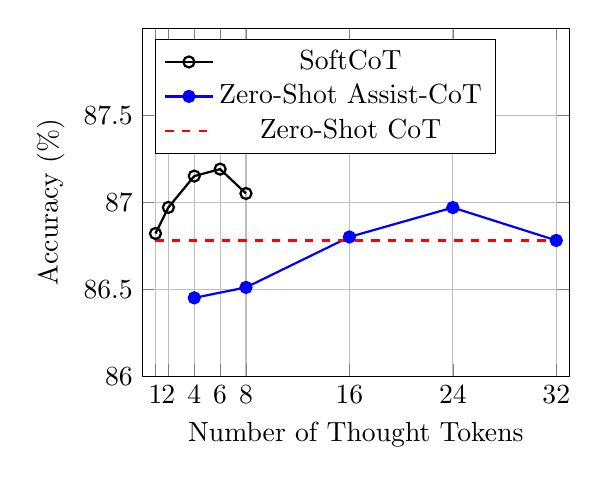
\begin{tikzpicture}
      \begin{axis}[
          width=7cm, height=6cm,
          xlabel={Number of Thought Tokens},
          ylabel={Accuracy (\%)},
          xmin=0, xmax=33,
          ymin=86, ymax=88,
          xtick={1,2,4,6,8,16,24,32},
          ytick={86.0, 86.5, 87.0, 87.5},
          grid=major,
          legend pos=north west,
          every axis plot/.append style={thick}
      ]

      \addplot[color=black, mark=o] coordinates {(1, 86.82) (2, 86.97) (4, 87.15) (6, 87.19) (8, 87.05)};
      \addlegendentry{SoftCoT};

      \addplot[color=blue, mark=*] coordinates {(4, 86.45) (8, 86.51) (16, 86.80) (24, 86.969) (32, 86.78)};
      \addlegendentry{Zero-Shot Assist-CoT};

      \addplot[color=red, dashed] coordinates {(1, 86.78) (32, 86.78)};
      \addlegendentry{Zero-Shot CoT};


      \end{axis}
  \end{tikzpicture}
  \caption{The impact of thought token numbers in ASDiv-Aug using LLaMA-3.1-8B-Instruct.}
  \label{fig:softcot-exp-num-thought-tokens}
\end{figure}


\subsubsection{Model-Related Factors}

To better understand SoftCoT, we conduct experiments to examine the impact of the number of thought tokens. The results, presented in Figure~\ref{fig:softcot-exp-num-thought-tokens}, lead to the following key observations:

\noindent (1) {\bf Soft thoughts reduce the required number of thought tokens}: We observe that SoftCoT achieves optimal performance with only six thought tokens, whereas Zero-Shot Assist-CoT requires 24 thought tokens to reach a similar level of effectiveness. This suggests that soft thoughts, which operate in a continuous space, exhibit a stronger representational capacity than hard thoughts expressed in the discrete language space. Our experiments indicate that the optimal number of hard thought tokens is approximately four times that of soft thought tokens, aligning with the 5x ratio reported by \citet{DBLP:journals/corr/abs-2412-13171}.


\noindent (2) {\bf SoftCoT mitigates the catastrophic forgetting problem}: Experimental results show that SoftCoT consistently outperforms Zero-Shot CoT across all tested numbers of soft thought tokens. In contrast, Zero-Shot Assist-CoT underperforms compared to Zero-Shot CoT when the number of thought tokens is insufficient. This is likely because the assistant model fails to generate a sufficiently informative set of thought tokens under these constraints, introducing noise and leading to confusion in the LLM's reasoning process.


\subsubsection{Model-Orthogonal Factors}

Self-Consistency~\cite{DBLP:conf/iclr/0002WSLCNCZ23} is a widely adopted technique for enhancing Chain-of-Thought (CoT) reasoning by expanding the search space. One of the most straightforward implementations involves generating multiple CoT reasoning paths and determining the final answer through majority voting. This approach is effective in mitigating errors in reasoning steps by leveraging the diversity of generated thought processes.

To further assess the effectiveness of SoftCoT, we conduct experiments incorporating self-consistency. As shown in Table~\ref{table:softcot-experiment-self-consistency}, SoftCoT consistently outperforms baseline models, demonstrating that its benefits are complementary to those of self-consistency rather than being redundant or conflicting. This suggests that SoftCoT introduces an independent improvement mechanism, which can be effectively combined with self-consistency for enhanced reasoning performance.

A key advantage of SoftCoT in this context is its ability to provide a more expressive and compact representation of intermediate reasoning steps in continuous space. Unlike traditional CoT reasoning, where discrete thought tokens may introduce inconsistencies or redundant reasoning paths, SoftCoT enables more efficient reasoning trajectories with fewer tokens. This allows self-consistency methods to aggregate results from higher-quality reasoning paths, leading to a more robust and accurate final prediction.


\begin{table}[t!]
    \centering
    \tabcolsep 6.0pt
    \begin{tabular}{l| c c}
    \toprule
    Model & $N=1$ & $N=10$\\
    \midrule
    Zero-Shot CoT & 79.61 & 90.37 \\
    Zero-Shot CoT-Unk & 79.95 & 90.43 \\
    Zero-Shot Assist-CoT & 80.76 & 90.54 \\
    \midrule
    SoftCoT & {\bf 81.03} & {\bf 90.98} \\
    \bottomrule
\end{tabular}
    \caption{Self Consistency for SoftCoT on LLaMA-3.1-8B-Instruct. ``$N$'' indicates the number of reasoning chains.}\label{table:softcot-experiment-self-consistency}
\end{table}



\section{Conclusion}

In this paper, we introduce SoftCoT, a soft chain-of-thought prompting approach for efficient LLM reasoning. SoftCoT consists of three steps: (1) an assistant model generates soft thought tokens, (2) a projection module trained to map the soft thoughts to LLM's representation space, and (3) the LLM applies soft thoughts for reasoning. To enhance efficiency, SoftCoT speculatively generates \textit{all} the soft thought tokens in a single forward pass. To mitigate the catastrophic forgetting, SoftCoT freezes the backbone LLM and only tunes the projection module. Experiments on five datasets across three types of reason tasks demonstrate the effectiveness of our proposed SoftCoT. Experiments on multiple LLMs as well as orthogonal method such as self-consistency shows the robustness of SoftCoT, which can be adapted in widely scenarios.


\section*{Limitations}
While SoftCoT represents a promising advancement in Chain-of-Thought (CoT) reasoning within a continuous space, several limitations must be acknowledged.

\paragraph{SoftCoT Cannot Fully Replace the Reasoning Path}: Although SoftCoT employs soft thought tokens for reasoning, it does not entirely replace the reasoning path. The decoding stage functions as a search process, which is a crucial component of CoT reasoning. Soft thought tokens primarily serve to enrich the probability space for exploration rather than acting as the search mechanism itself.

\paragraph{Need for Further Empirical Evidence on Scalability}: SoftCoT has been evaluated on LLaMA-3.1-8B-Instruct and Qwen2.5-7B-Instruct. However, larger backbone LLMs exist within the same model families. While its success on models with approximately 7–8 billion parameters suggests potential applicability to larger-scale models, its scalability to extremely large LLMs remains an open question and requires thorough empirical validation.



% \section*{Ethics Statement}
% Scientific work published at ACL 2023 must comply with the ACL Ethics Policy.\footnote{\url{https://www.aclweb.org/portal/content/acl-code-ethics}} We encourage all authors to include an explicit ethics statement on the broader impact of the work, or other ethical considerations after the conclusion but before the references. The ethics statement will not count toward the page limit (8 pages for long, 4 pages for short papers).

% \section*{Acknowledgements}
% This document has been adapted by Jordan Boyd-Graber, Naoaki Okazaki, Anna Rogers from the style files used for earlier ACL, EMNLP and NAACL proceedings, including those for
% EACL 2023 by Isabelle Augenstein and Andreas Vlachos,
% EMNLP 2022 by Yue Zhang, Ryan Cotterell and Lea Frermann,
% ACL 2020 by Steven Bethard, Ryan Cotterell and Rui Yan,
% ACL 2019 by Douwe Kiela and Ivan Vuli\'{c},
% NAACL 2019 by Stephanie Lukin and Alla Roskovskaya,
% ACL 2018 by Shay Cohen, Kevin Gimpel, and Wei Lu,
% NAACL 2018 by Margaret Mitchell and Stephanie Lukin,
% Bib\TeX{} suggestions for (NA)ACL 2017/2018 from Jason Eisner,
% ACL 2017 by Dan Gildea and Min-Yen Kan, NAACL 2017 by Margaret Mitchell,
% ACL 2012 by Maggie Li and Michael White,
% ACL 2010 by Jing-Shin Chang and Philipp Koehn,
% ACL 2008 by Johanna D. Moore, Simone Teufel, James Allan, and Sadaoki Furui,
% ACL 2005 by Hwee Tou Ng and Kemal Oflazer,
% ACL 2002 by Eugene Charniak and Dekang Lin,
% and earlier ACL and EACL formats written by several people, including
% John Chen, Henry S. Thompson and Donald Walker.
% Additional elements were taken from the formatting instructions of the \emph{International Joint Conference on Artificial Intelligence} and the \emph{Conference on Computer Vision and Pattern Recognition}.

% Entries for the entire Anthology, followed by custom entries
\bibliography{nlp}
\bibliographystyle{acl_natbib}


\appendix

\subsection{Lloyd-Max Algorithm}
\label{subsec:Lloyd-Max}
For a given quantization bitwidth $B$ and an operand $\bm{X}$, the Lloyd-Max algorithm finds $2^B$ quantization levels $\{\hat{x}_i\}_{i=1}^{2^B}$ such that quantizing $\bm{X}$ by rounding each scalar in $\bm{X}$ to the nearest quantization level minimizes the quantization MSE. 

The algorithm starts with an initial guess of quantization levels and then iteratively computes quantization thresholds $\{\tau_i\}_{i=1}^{2^B-1}$ and updates quantization levels $\{\hat{x}_i\}_{i=1}^{2^B}$. Specifically, at iteration $n$, thresholds are set to the midpoints of the previous iteration's levels:
\begin{align*}
    \tau_i^{(n)}=\frac{\hat{x}_i^{(n-1)}+\hat{x}_{i+1}^{(n-1)}}2 \text{ for } i=1\ldots 2^B-1
\end{align*}
Subsequently, the quantization levels are re-computed as conditional means of the data regions defined by the new thresholds:
\begin{align*}
    \hat{x}_i^{(n)}=\mathbb{E}\left[ \bm{X} \big| \bm{X}\in [\tau_{i-1}^{(n)},\tau_i^{(n)}] \right] \text{ for } i=1\ldots 2^B
\end{align*}
where to satisfy boundary conditions we have $\tau_0=-\infty$ and $\tau_{2^B}=\infty$. The algorithm iterates the above steps until convergence.

Figure \ref{fig:lm_quant} compares the quantization levels of a $7$-bit floating point (E3M3) quantizer (left) to a $7$-bit Lloyd-Max quantizer (right) when quantizing a layer of weights from the GPT3-126M model at a per-tensor granularity. As shown, the Lloyd-Max quantizer achieves substantially lower quantization MSE. Further, Table \ref{tab:FP7_vs_LM7} shows the superior perplexity achieved by Lloyd-Max quantizers for bitwidths of $7$, $6$ and $5$. The difference between the quantizers is clear at 5 bits, where per-tensor FP quantization incurs a drastic and unacceptable increase in perplexity, while Lloyd-Max quantization incurs a much smaller increase. Nevertheless, we note that even the optimal Lloyd-Max quantizer incurs a notable ($\sim 1.5$) increase in perplexity due to the coarse granularity of quantization. 

\begin{figure}[h]
  \centering
  \includegraphics[width=0.7\linewidth]{sections/figures/LM7_FP7.pdf}
  \caption{\small Quantization levels and the corresponding quantization MSE of Floating Point (left) vs Lloyd-Max (right) Quantizers for a layer of weights in the GPT3-126M model.}
  \label{fig:lm_quant}
\end{figure}

\begin{table}[h]\scriptsize
\begin{center}
\caption{\label{tab:FP7_vs_LM7} \small Comparing perplexity (lower is better) achieved by floating point quantizers and Lloyd-Max quantizers on a GPT3-126M model for the Wikitext-103 dataset.}
\begin{tabular}{c|cc|c}
\hline
 \multirow{2}{*}{\textbf{Bitwidth}} & \multicolumn{2}{|c|}{\textbf{Floating-Point Quantizer}} & \textbf{Lloyd-Max Quantizer} \\
 & Best Format & Wikitext-103 Perplexity & Wikitext-103 Perplexity \\
\hline
7 & E3M3 & 18.32 & 18.27 \\
6 & E3M2 & 19.07 & 18.51 \\
5 & E4M0 & 43.89 & 19.71 \\
\hline
\end{tabular}
\end{center}
\end{table}

\subsection{Proof of Local Optimality of LO-BCQ}
\label{subsec:lobcq_opt_proof}
For a given block $\bm{b}_j$, the quantization MSE during LO-BCQ can be empirically evaluated as $\frac{1}{L_b}\lVert \bm{b}_j- \bm{\hat{b}}_j\rVert^2_2$ where $\bm{\hat{b}}_j$ is computed from equation (\ref{eq:clustered_quantization_definition}) as $C_{f(\bm{b}_j)}(\bm{b}_j)$. Further, for a given block cluster $\mathcal{B}_i$, we compute the quantization MSE as $\frac{1}{|\mathcal{B}_{i}|}\sum_{\bm{b} \in \mathcal{B}_{i}} \frac{1}{L_b}\lVert \bm{b}- C_i^{(n)}(\bm{b})\rVert^2_2$. Therefore, at the end of iteration $n$, we evaluate the overall quantization MSE $J^{(n)}$ for a given operand $\bm{X}$ composed of $N_c$ block clusters as:
\begin{align*}
    \label{eq:mse_iter_n}
    J^{(n)} = \frac{1}{N_c} \sum_{i=1}^{N_c} \frac{1}{|\mathcal{B}_{i}^{(n)}|}\sum_{\bm{v} \in \mathcal{B}_{i}^{(n)}} \frac{1}{L_b}\lVert \bm{b}- B_i^{(n)}(\bm{b})\rVert^2_2
\end{align*}

At the end of iteration $n$, the codebooks are updated from $\mathcal{C}^{(n-1)}$ to $\mathcal{C}^{(n)}$. However, the mapping of a given vector $\bm{b}_j$ to quantizers $\mathcal{C}^{(n)}$ remains as  $f^{(n)}(\bm{b}_j)$. At the next iteration, during the vector clustering step, $f^{(n+1)}(\bm{b}_j)$ finds new mapping of $\bm{b}_j$ to updated codebooks $\mathcal{C}^{(n)}$ such that the quantization MSE over the candidate codebooks is minimized. Therefore, we obtain the following result for $\bm{b}_j$:
\begin{align*}
\frac{1}{L_b}\lVert \bm{b}_j - C_{f^{(n+1)}(\bm{b}_j)}^{(n)}(\bm{b}_j)\rVert^2_2 \le \frac{1}{L_b}\lVert \bm{b}_j - C_{f^{(n)}(\bm{b}_j)}^{(n)}(\bm{b}_j)\rVert^2_2
\end{align*}

That is, quantizing $\bm{b}_j$ at the end of the block clustering step of iteration $n+1$ results in lower quantization MSE compared to quantizing at the end of iteration $n$. Since this is true for all $\bm{b} \in \bm{X}$, we assert the following:
\begin{equation}
\begin{split}
\label{eq:mse_ineq_1}
    \tilde{J}^{(n+1)} &= \frac{1}{N_c} \sum_{i=1}^{N_c} \frac{1}{|\mathcal{B}_{i}^{(n+1)}|}\sum_{\bm{b} \in \mathcal{B}_{i}^{(n+1)}} \frac{1}{L_b}\lVert \bm{b} - C_i^{(n)}(b)\rVert^2_2 \le J^{(n)}
\end{split}
\end{equation}
where $\tilde{J}^{(n+1)}$ is the the quantization MSE after the vector clustering step at iteration $n+1$.

Next, during the codebook update step (\ref{eq:quantizers_update}) at iteration $n+1$, the per-cluster codebooks $\mathcal{C}^{(n)}$ are updated to $\mathcal{C}^{(n+1)}$ by invoking the Lloyd-Max algorithm \citep{Lloyd}. We know that for any given value distribution, the Lloyd-Max algorithm minimizes the quantization MSE. Therefore, for a given vector cluster $\mathcal{B}_i$ we obtain the following result:

\begin{equation}
    \frac{1}{|\mathcal{B}_{i}^{(n+1)}|}\sum_{\bm{b} \in \mathcal{B}_{i}^{(n+1)}} \frac{1}{L_b}\lVert \bm{b}- C_i^{(n+1)}(\bm{b})\rVert^2_2 \le \frac{1}{|\mathcal{B}_{i}^{(n+1)}|}\sum_{\bm{b} \in \mathcal{B}_{i}^{(n+1)}} \frac{1}{L_b}\lVert \bm{b}- C_i^{(n)}(\bm{b})\rVert^2_2
\end{equation}

The above equation states that quantizing the given block cluster $\mathcal{B}_i$ after updating the associated codebook from $C_i^{(n)}$ to $C_i^{(n+1)}$ results in lower quantization MSE. Since this is true for all the block clusters, we derive the following result: 
\begin{equation}
\begin{split}
\label{eq:mse_ineq_2}
     J^{(n+1)} &= \frac{1}{N_c} \sum_{i=1}^{N_c} \frac{1}{|\mathcal{B}_{i}^{(n+1)}|}\sum_{\bm{b} \in \mathcal{B}_{i}^{(n+1)}} \frac{1}{L_b}\lVert \bm{b}- C_i^{(n+1)}(\bm{b})\rVert^2_2  \le \tilde{J}^{(n+1)}   
\end{split}
\end{equation}

Following (\ref{eq:mse_ineq_1}) and (\ref{eq:mse_ineq_2}), we find that the quantization MSE is non-increasing for each iteration, that is, $J^{(1)} \ge J^{(2)} \ge J^{(3)} \ge \ldots \ge J^{(M)}$ where $M$ is the maximum number of iterations. 
%Therefore, we can say that if the algorithm converges, then it must be that it has converged to a local minimum. 
\hfill $\blacksquare$


\begin{figure}
    \begin{center}
    \includegraphics[width=0.5\textwidth]{sections//figures/mse_vs_iter.pdf}
    \end{center}
    \caption{\small NMSE vs iterations during LO-BCQ compared to other block quantization proposals}
    \label{fig:nmse_vs_iter}
\end{figure}

Figure \ref{fig:nmse_vs_iter} shows the empirical convergence of LO-BCQ across several block lengths and number of codebooks. Also, the MSE achieved by LO-BCQ is compared to baselines such as MXFP and VSQ. As shown, LO-BCQ converges to a lower MSE than the baselines. Further, we achieve better convergence for larger number of codebooks ($N_c$) and for a smaller block length ($L_b$), both of which increase the bitwidth of BCQ (see Eq \ref{eq:bitwidth_bcq}).


\subsection{Additional Accuracy Results}
%Table \ref{tab:lobcq_config} lists the various LOBCQ configurations and their corresponding bitwidths.
\begin{table}
\setlength{\tabcolsep}{4.75pt}
\begin{center}
\caption{\label{tab:lobcq_config} Various LO-BCQ configurations and their bitwidths.}
\begin{tabular}{|c||c|c|c|c||c|c||c|} 
\hline
 & \multicolumn{4}{|c||}{$L_b=8$} & \multicolumn{2}{|c||}{$L_b=4$} & $L_b=2$ \\
 \hline
 \backslashbox{$L_A$\kern-1em}{\kern-1em$N_c$} & 2 & 4 & 8 & 16 & 2 & 4 & 2 \\
 \hline
 64 & 4.25 & 4.375 & 4.5 & 4.625 & 4.375 & 4.625 & 4.625\\
 \hline
 32 & 4.375 & 4.5 & 4.625& 4.75 & 4.5 & 4.75 & 4.75 \\
 \hline
 16 & 4.625 & 4.75& 4.875 & 5 & 4.75 & 5 & 5 \\
 \hline
\end{tabular}
\end{center}
\end{table}

%\subsection{Perplexity achieved by various LO-BCQ configurations on Wikitext-103 dataset}

\begin{table} \centering
\begin{tabular}{|c||c|c|c|c||c|c||c|} 
\hline
 $L_b \rightarrow$& \multicolumn{4}{c||}{8} & \multicolumn{2}{c||}{4} & 2\\
 \hline
 \backslashbox{$L_A$\kern-1em}{\kern-1em$N_c$} & 2 & 4 & 8 & 16 & 2 & 4 & 2  \\
 %$N_c \rightarrow$ & 2 & 4 & 8 & 16 & 2 & 4 & 2 \\
 \hline
 \hline
 \multicolumn{8}{c}{GPT3-1.3B (FP32 PPL = 9.98)} \\ 
 \hline
 \hline
 64 & 10.40 & 10.23 & 10.17 & 10.15 &  10.28 & 10.18 & 10.19 \\
 \hline
 32 & 10.25 & 10.20 & 10.15 & 10.12 &  10.23 & 10.17 & 10.17 \\
 \hline
 16 & 10.22 & 10.16 & 10.10 & 10.09 &  10.21 & 10.14 & 10.16 \\
 \hline
  \hline
 \multicolumn{8}{c}{GPT3-8B (FP32 PPL = 7.38)} \\ 
 \hline
 \hline
 64 & 7.61 & 7.52 & 7.48 &  7.47 &  7.55 &  7.49 & 7.50 \\
 \hline
 32 & 7.52 & 7.50 & 7.46 &  7.45 &  7.52 &  7.48 & 7.48  \\
 \hline
 16 & 7.51 & 7.48 & 7.44 &  7.44 &  7.51 &  7.49 & 7.47  \\
 \hline
\end{tabular}
\caption{\label{tab:ppl_gpt3_abalation} Wikitext-103 perplexity across GPT3-1.3B and 8B models.}
\end{table}

\begin{table} \centering
\begin{tabular}{|c||c|c|c|c||} 
\hline
 $L_b \rightarrow$& \multicolumn{4}{c||}{8}\\
 \hline
 \backslashbox{$L_A$\kern-1em}{\kern-1em$N_c$} & 2 & 4 & 8 & 16 \\
 %$N_c \rightarrow$ & 2 & 4 & 8 & 16 & 2 & 4 & 2 \\
 \hline
 \hline
 \multicolumn{5}{|c|}{Llama2-7B (FP32 PPL = 5.06)} \\ 
 \hline
 \hline
 64 & 5.31 & 5.26 & 5.19 & 5.18  \\
 \hline
 32 & 5.23 & 5.25 & 5.18 & 5.15  \\
 \hline
 16 & 5.23 & 5.19 & 5.16 & 5.14  \\
 \hline
 \multicolumn{5}{|c|}{Nemotron4-15B (FP32 PPL = 5.87)} \\ 
 \hline
 \hline
 64  & 6.3 & 6.20 & 6.13 & 6.08  \\
 \hline
 32  & 6.24 & 6.12 & 6.07 & 6.03  \\
 \hline
 16  & 6.12 & 6.14 & 6.04 & 6.02  \\
 \hline
 \multicolumn{5}{|c|}{Nemotron4-340B (FP32 PPL = 3.48)} \\ 
 \hline
 \hline
 64 & 3.67 & 3.62 & 3.60 & 3.59 \\
 \hline
 32 & 3.63 & 3.61 & 3.59 & 3.56 \\
 \hline
 16 & 3.61 & 3.58 & 3.57 & 3.55 \\
 \hline
\end{tabular}
\caption{\label{tab:ppl_llama7B_nemo15B} Wikitext-103 perplexity compared to FP32 baseline in Llama2-7B and Nemotron4-15B, 340B models}
\end{table}

%\subsection{Perplexity achieved by various LO-BCQ configurations on MMLU dataset}


\begin{table} \centering
\begin{tabular}{|c||c|c|c|c||c|c|c|c|} 
\hline
 $L_b \rightarrow$& \multicolumn{4}{c||}{8} & \multicolumn{4}{c||}{8}\\
 \hline
 \backslashbox{$L_A$\kern-1em}{\kern-1em$N_c$} & 2 & 4 & 8 & 16 & 2 & 4 & 8 & 16  \\
 %$N_c \rightarrow$ & 2 & 4 & 8 & 16 & 2 & 4 & 2 \\
 \hline
 \hline
 \multicolumn{5}{|c|}{Llama2-7B (FP32 Accuracy = 45.8\%)} & \multicolumn{4}{|c|}{Llama2-70B (FP32 Accuracy = 69.12\%)} \\ 
 \hline
 \hline
 64 & 43.9 & 43.4 & 43.9 & 44.9 & 68.07 & 68.27 & 68.17 & 68.75 \\
 \hline
 32 & 44.5 & 43.8 & 44.9 & 44.5 & 68.37 & 68.51 & 68.35 & 68.27  \\
 \hline
 16 & 43.9 & 42.7 & 44.9 & 45 & 68.12 & 68.77 & 68.31 & 68.59  \\
 \hline
 \hline
 \multicolumn{5}{|c|}{GPT3-22B (FP32 Accuracy = 38.75\%)} & \multicolumn{4}{|c|}{Nemotron4-15B (FP32 Accuracy = 64.3\%)} \\ 
 \hline
 \hline
 64 & 36.71 & 38.85 & 38.13 & 38.92 & 63.17 & 62.36 & 63.72 & 64.09 \\
 \hline
 32 & 37.95 & 38.69 & 39.45 & 38.34 & 64.05 & 62.30 & 63.8 & 64.33  \\
 \hline
 16 & 38.88 & 38.80 & 38.31 & 38.92 & 63.22 & 63.51 & 63.93 & 64.43  \\
 \hline
\end{tabular}
\caption{\label{tab:mmlu_abalation} Accuracy on MMLU dataset across GPT3-22B, Llama2-7B, 70B and Nemotron4-15B models.}
\end{table}


%\subsection{Perplexity achieved by various LO-BCQ configurations on LM evaluation harness}

\begin{table} \centering
\begin{tabular}{|c||c|c|c|c||c|c|c|c|} 
\hline
 $L_b \rightarrow$& \multicolumn{4}{c||}{8} & \multicolumn{4}{c||}{8}\\
 \hline
 \backslashbox{$L_A$\kern-1em}{\kern-1em$N_c$} & 2 & 4 & 8 & 16 & 2 & 4 & 8 & 16  \\
 %$N_c \rightarrow$ & 2 & 4 & 8 & 16 & 2 & 4 & 2 \\
 \hline
 \hline
 \multicolumn{5}{|c|}{Race (FP32 Accuracy = 37.51\%)} & \multicolumn{4}{|c|}{Boolq (FP32 Accuracy = 64.62\%)} \\ 
 \hline
 \hline
 64 & 36.94 & 37.13 & 36.27 & 37.13 & 63.73 & 62.26 & 63.49 & 63.36 \\
 \hline
 32 & 37.03 & 36.36 & 36.08 & 37.03 & 62.54 & 63.51 & 63.49 & 63.55  \\
 \hline
 16 & 37.03 & 37.03 & 36.46 & 37.03 & 61.1 & 63.79 & 63.58 & 63.33  \\
 \hline
 \hline
 \multicolumn{5}{|c|}{Winogrande (FP32 Accuracy = 58.01\%)} & \multicolumn{4}{|c|}{Piqa (FP32 Accuracy = 74.21\%)} \\ 
 \hline
 \hline
 64 & 58.17 & 57.22 & 57.85 & 58.33 & 73.01 & 73.07 & 73.07 & 72.80 \\
 \hline
 32 & 59.12 & 58.09 & 57.85 & 58.41 & 73.01 & 73.94 & 72.74 & 73.18  \\
 \hline
 16 & 57.93 & 58.88 & 57.93 & 58.56 & 73.94 & 72.80 & 73.01 & 73.94  \\
 \hline
\end{tabular}
\caption{\label{tab:mmlu_abalation} Accuracy on LM evaluation harness tasks on GPT3-1.3B model.}
\end{table}

\begin{table} \centering
\begin{tabular}{|c||c|c|c|c||c|c|c|c|} 
\hline
 $L_b \rightarrow$& \multicolumn{4}{c||}{8} & \multicolumn{4}{c||}{8}\\
 \hline
 \backslashbox{$L_A$\kern-1em}{\kern-1em$N_c$} & 2 & 4 & 8 & 16 & 2 & 4 & 8 & 16  \\
 %$N_c \rightarrow$ & 2 & 4 & 8 & 16 & 2 & 4 & 2 \\
 \hline
 \hline
 \multicolumn{5}{|c|}{Race (FP32 Accuracy = 41.34\%)} & \multicolumn{4}{|c|}{Boolq (FP32 Accuracy = 68.32\%)} \\ 
 \hline
 \hline
 64 & 40.48 & 40.10 & 39.43 & 39.90 & 69.20 & 68.41 & 69.45 & 68.56 \\
 \hline
 32 & 39.52 & 39.52 & 40.77 & 39.62 & 68.32 & 67.43 & 68.17 & 69.30  \\
 \hline
 16 & 39.81 & 39.71 & 39.90 & 40.38 & 68.10 & 66.33 & 69.51 & 69.42  \\
 \hline
 \hline
 \multicolumn{5}{|c|}{Winogrande (FP32 Accuracy = 67.88\%)} & \multicolumn{4}{|c|}{Piqa (FP32 Accuracy = 78.78\%)} \\ 
 \hline
 \hline
 64 & 66.85 & 66.61 & 67.72 & 67.88 & 77.31 & 77.42 & 77.75 & 77.64 \\
 \hline
 32 & 67.25 & 67.72 & 67.72 & 67.00 & 77.31 & 77.04 & 77.80 & 77.37  \\
 \hline
 16 & 68.11 & 68.90 & 67.88 & 67.48 & 77.37 & 78.13 & 78.13 & 77.69  \\
 \hline
\end{tabular}
\caption{\label{tab:mmlu_abalation} Accuracy on LM evaluation harness tasks on GPT3-8B model.}
\end{table}

\begin{table} \centering
\begin{tabular}{|c||c|c|c|c||c|c|c|c|} 
\hline
 $L_b \rightarrow$& \multicolumn{4}{c||}{8} & \multicolumn{4}{c||}{8}\\
 \hline
 \backslashbox{$L_A$\kern-1em}{\kern-1em$N_c$} & 2 & 4 & 8 & 16 & 2 & 4 & 8 & 16  \\
 %$N_c \rightarrow$ & 2 & 4 & 8 & 16 & 2 & 4 & 2 \\
 \hline
 \hline
 \multicolumn{5}{|c|}{Race (FP32 Accuracy = 40.67\%)} & \multicolumn{4}{|c|}{Boolq (FP32 Accuracy = 76.54\%)} \\ 
 \hline
 \hline
 64 & 40.48 & 40.10 & 39.43 & 39.90 & 75.41 & 75.11 & 77.09 & 75.66 \\
 \hline
 32 & 39.52 & 39.52 & 40.77 & 39.62 & 76.02 & 76.02 & 75.96 & 75.35  \\
 \hline
 16 & 39.81 & 39.71 & 39.90 & 40.38 & 75.05 & 73.82 & 75.72 & 76.09  \\
 \hline
 \hline
 \multicolumn{5}{|c|}{Winogrande (FP32 Accuracy = 70.64\%)} & \multicolumn{4}{|c|}{Piqa (FP32 Accuracy = 79.16\%)} \\ 
 \hline
 \hline
 64 & 69.14 & 70.17 & 70.17 & 70.56 & 78.24 & 79.00 & 78.62 & 78.73 \\
 \hline
 32 & 70.96 & 69.69 & 71.27 & 69.30 & 78.56 & 79.49 & 79.16 & 78.89  \\
 \hline
 16 & 71.03 & 69.53 & 69.69 & 70.40 & 78.13 & 79.16 & 79.00 & 79.00  \\
 \hline
\end{tabular}
\caption{\label{tab:mmlu_abalation} Accuracy on LM evaluation harness tasks on GPT3-22B model.}
\end{table}

\begin{table} \centering
\begin{tabular}{|c||c|c|c|c||c|c|c|c|} 
\hline
 $L_b \rightarrow$& \multicolumn{4}{c||}{8} & \multicolumn{4}{c||}{8}\\
 \hline
 \backslashbox{$L_A$\kern-1em}{\kern-1em$N_c$} & 2 & 4 & 8 & 16 & 2 & 4 & 8 & 16  \\
 %$N_c \rightarrow$ & 2 & 4 & 8 & 16 & 2 & 4 & 2 \\
 \hline
 \hline
 \multicolumn{5}{|c|}{Race (FP32 Accuracy = 44.4\%)} & \multicolumn{4}{|c|}{Boolq (FP32 Accuracy = 79.29\%)} \\ 
 \hline
 \hline
 64 & 42.49 & 42.51 & 42.58 & 43.45 & 77.58 & 77.37 & 77.43 & 78.1 \\
 \hline
 32 & 43.35 & 42.49 & 43.64 & 43.73 & 77.86 & 75.32 & 77.28 & 77.86  \\
 \hline
 16 & 44.21 & 44.21 & 43.64 & 42.97 & 78.65 & 77 & 76.94 & 77.98  \\
 \hline
 \hline
 \multicolumn{5}{|c|}{Winogrande (FP32 Accuracy = 69.38\%)} & \multicolumn{4}{|c|}{Piqa (FP32 Accuracy = 78.07\%)} \\ 
 \hline
 \hline
 64 & 68.9 & 68.43 & 69.77 & 68.19 & 77.09 & 76.82 & 77.09 & 77.86 \\
 \hline
 32 & 69.38 & 68.51 & 68.82 & 68.90 & 78.07 & 76.71 & 78.07 & 77.86  \\
 \hline
 16 & 69.53 & 67.09 & 69.38 & 68.90 & 77.37 & 77.8 & 77.91 & 77.69  \\
 \hline
\end{tabular}
\caption{\label{tab:mmlu_abalation} Accuracy on LM evaluation harness tasks on Llama2-7B model.}
\end{table}

\begin{table} \centering
\begin{tabular}{|c||c|c|c|c||c|c|c|c|} 
\hline
 $L_b \rightarrow$& \multicolumn{4}{c||}{8} & \multicolumn{4}{c||}{8}\\
 \hline
 \backslashbox{$L_A$\kern-1em}{\kern-1em$N_c$} & 2 & 4 & 8 & 16 & 2 & 4 & 8 & 16  \\
 %$N_c \rightarrow$ & 2 & 4 & 8 & 16 & 2 & 4 & 2 \\
 \hline
 \hline
 \multicolumn{5}{|c|}{Race (FP32 Accuracy = 48.8\%)} & \multicolumn{4}{|c|}{Boolq (FP32 Accuracy = 85.23\%)} \\ 
 \hline
 \hline
 64 & 49.00 & 49.00 & 49.28 & 48.71 & 82.82 & 84.28 & 84.03 & 84.25 \\
 \hline
 32 & 49.57 & 48.52 & 48.33 & 49.28 & 83.85 & 84.46 & 84.31 & 84.93  \\
 \hline
 16 & 49.85 & 49.09 & 49.28 & 48.99 & 85.11 & 84.46 & 84.61 & 83.94  \\
 \hline
 \hline
 \multicolumn{5}{|c|}{Winogrande (FP32 Accuracy = 79.95\%)} & \multicolumn{4}{|c|}{Piqa (FP32 Accuracy = 81.56\%)} \\ 
 \hline
 \hline
 64 & 78.77 & 78.45 & 78.37 & 79.16 & 81.45 & 80.69 & 81.45 & 81.5 \\
 \hline
 32 & 78.45 & 79.01 & 78.69 & 80.66 & 81.56 & 80.58 & 81.18 & 81.34  \\
 \hline
 16 & 79.95 & 79.56 & 79.79 & 79.72 & 81.28 & 81.66 & 81.28 & 80.96  \\
 \hline
\end{tabular}
\caption{\label{tab:mmlu_abalation} Accuracy on LM evaluation harness tasks on Llama2-70B model.}
\end{table}

%\section{MSE Studies}
%\textcolor{red}{TODO}


\subsection{Number Formats and Quantization Method}
\label{subsec:numFormats_quantMethod}
\subsubsection{Integer Format}
An $n$-bit signed integer (INT) is typically represented with a 2s-complement format \citep{yao2022zeroquant,xiao2023smoothquant,dai2021vsq}, where the most significant bit denotes the sign.

\subsubsection{Floating Point Format}
An $n$-bit signed floating point (FP) number $x$ comprises of a 1-bit sign ($x_{\mathrm{sign}}$), $B_m$-bit mantissa ($x_{\mathrm{mant}}$) and $B_e$-bit exponent ($x_{\mathrm{exp}}$) such that $B_m+B_e=n-1$. The associated constant exponent bias ($E_{\mathrm{bias}}$) is computed as $(2^{{B_e}-1}-1)$. We denote this format as $E_{B_e}M_{B_m}$.  

\subsubsection{Quantization Scheme}
\label{subsec:quant_method}
A quantization scheme dictates how a given unquantized tensor is converted to its quantized representation. We consider FP formats for the purpose of illustration. Given an unquantized tensor $\bm{X}$ and an FP format $E_{B_e}M_{B_m}$, we first, we compute the quantization scale factor $s_X$ that maps the maximum absolute value of $\bm{X}$ to the maximum quantization level of the $E_{B_e}M_{B_m}$ format as follows:
\begin{align}
\label{eq:sf}
    s_X = \frac{\mathrm{max}(|\bm{X}|)}{\mathrm{max}(E_{B_e}M_{B_m})}
\end{align}
In the above equation, $|\cdot|$ denotes the absolute value function.

Next, we scale $\bm{X}$ by $s_X$ and quantize it to $\hat{\bm{X}}$ by rounding it to the nearest quantization level of $E_{B_e}M_{B_m}$ as:

\begin{align}
\label{eq:tensor_quant}
    \hat{\bm{X}} = \text{round-to-nearest}\left(\frac{\bm{X}}{s_X}, E_{B_e}M_{B_m}\right)
\end{align}

We perform dynamic max-scaled quantization \citep{wu2020integer}, where the scale factor $s$ for activations is dynamically computed during runtime.

\subsection{Vector Scaled Quantization}
\begin{wrapfigure}{r}{0.35\linewidth}
  \centering
  \includegraphics[width=\linewidth]{sections/figures/vsquant.jpg}
  \caption{\small Vectorwise decomposition for per-vector scaled quantization (VSQ \citep{dai2021vsq}).}
  \label{fig:vsquant}
\end{wrapfigure}
During VSQ \citep{dai2021vsq}, the operand tensors are decomposed into 1D vectors in a hardware friendly manner as shown in Figure \ref{fig:vsquant}. Since the decomposed tensors are used as operands in matrix multiplications during inference, it is beneficial to perform this decomposition along the reduction dimension of the multiplication. The vectorwise quantization is performed similar to tensorwise quantization described in Equations \ref{eq:sf} and \ref{eq:tensor_quant}, where a scale factor $s_v$ is required for each vector $\bm{v}$ that maps the maximum absolute value of that vector to the maximum quantization level. While smaller vector lengths can lead to larger accuracy gains, the associated memory and computational overheads due to the per-vector scale factors increases. To alleviate these overheads, VSQ \citep{dai2021vsq} proposed a second level quantization of the per-vector scale factors to unsigned integers, while MX \citep{rouhani2023shared} quantizes them to integer powers of 2 (denoted as $2^{INT}$).

\subsubsection{MX Format}
The MX format proposed in \citep{rouhani2023microscaling} introduces the concept of sub-block shifting. For every two scalar elements of $b$-bits each, there is a shared exponent bit. The value of this exponent bit is determined through an empirical analysis that targets minimizing quantization MSE. We note that the FP format $E_{1}M_{b}$ is strictly better than MX from an accuracy perspective since it allocates a dedicated exponent bit to each scalar as opposed to sharing it across two scalars. Therefore, we conservatively bound the accuracy of a $b+2$-bit signed MX format with that of a $E_{1}M_{b}$ format in our comparisons. For instance, we use E1M2 format as a proxy for MX4.

\begin{figure}
    \centering
    \includegraphics[width=1\linewidth]{sections//figures/BlockFormats.pdf}
    \caption{\small Comparing LO-BCQ to MX format.}
    \label{fig:block_formats}
\end{figure}

Figure \ref{fig:block_formats} compares our $4$-bit LO-BCQ block format to MX \citep{rouhani2023microscaling}. As shown, both LO-BCQ and MX decompose a given operand tensor into block arrays and each block array into blocks. Similar to MX, we find that per-block quantization ($L_b < L_A$) leads to better accuracy due to increased flexibility. While MX achieves this through per-block $1$-bit micro-scales, we associate a dedicated codebook to each block through a per-block codebook selector. Further, MX quantizes the per-block array scale-factor to E8M0 format without per-tensor scaling. In contrast during LO-BCQ, we find that per-tensor scaling combined with quantization of per-block array scale-factor to E4M3 format results in superior inference accuracy across models. 

\end{document}
